\section{Casos de uso}

\subsection{\labeltext[UC00 - Sistema]{UC-00 - Sistema}{uc:00}}
A imagem identificada como figura~\ref{fig:chap210} apresenta o diagrama de caso de uso \ref{uc:00} e tem como objetivo ilustrar de modo geral como o sistema funcionará.

\vspace*{5mm}

\begin{figure}[H]
	\centering
	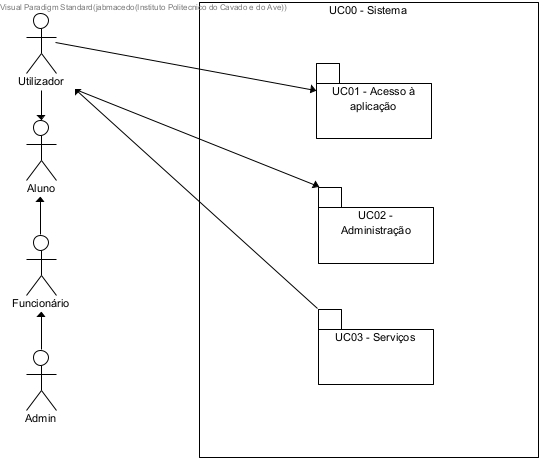
\includegraphics[width=1\linewidth]{./img/Diagramas\_UC/UC00.jpg}  % largura percentual 
	\caption{\ref{uc:00}}
	\label{fig:chap210}
\end{figure}

\par Tal como podemos observar na figura~\ref{fig:chap210}, consideramos que o nosso sistema está dividido em três grandes grupos de casos de uso, são:

\textbf{UC01 - Acesso a aplicação}  Aqui, iremos tratar os casos de uso referentes ao acesso à aplicação, tal como a criação de conta e autenticação do utilizador.

\textbf{UC02 - Administração}  Neste grupo, serão analisados os casos de uso referentes à gestão de conta e gestão de livros.

\textbf{UC03 - Serviços}  Para os serviços, tal como o nome indica iremos tratar abordar os casos de uso referente às requisições de livros, constultas e gestão de coimas.